%
% part1.tex
%

\section{Histogram-based Processing}

% 1.1
\subsection{CDF in relation to PDF}
The cumulative distribution function is the integral of the probabililty
density function. It calculates the cumulative probability of intensity values
in the interval $[0;x]$, for a given $x$.

% 1.2
\subsection{Constant images}
Under the assumption that a constant image refers to an image of unchanging
signal --- that is, an image consisting of a repeating pixel intensity. This
would mean that the probability density at $p_x(k) = 1$ for $k$, whilst
$\forall i \neq k (p_x(i) = 0)$. This would make a histogram with exactly one
spike at $x=k$, and a cumulative distribution curve that would be zero for all
$x < k$, and 1 for all $x \geq k$.

% 1.3
\subsection{Implementing cumulative histogram}
As we can see from the rendition of the histogram and the cumulative histogram
shown in figure \ref{fig:1-3} there are two regions of fast increase in the
curve, which indicate an increase in light of the image. Similarly, the flat
region indicate a steady intensity signal.

\begin{figure}[H]
    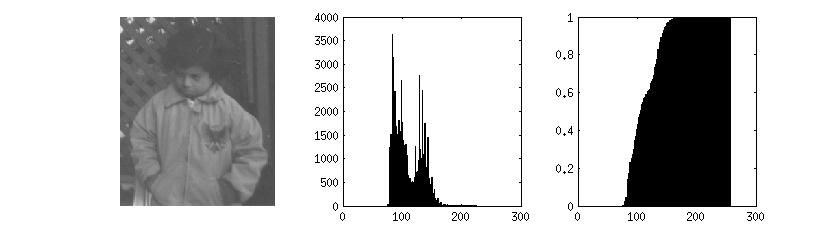
\includegraphics[scale=0.5]{figures/1-3.jpg}
    \caption{Original (left), histogram (middle) and cumulative histogram
    (right)}
    \label{fig:1-3}
\end{figure}

The code used to generate the figure is given in \ref{appendix:histcum}.

% 1.4
\subsection{Floating-point Image CDF}
\begin{multicols}{2}

    The code is given in \ref{appendix:fpimg}.
    
    \vfill{\ }\columnbreak
    
    \begin{figure}[H]
        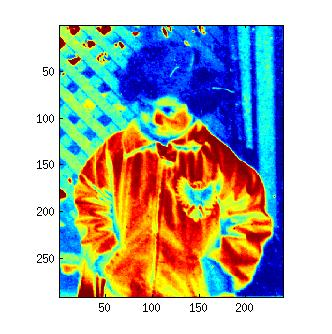
\includegraphics[scale=0.5]{figures/1-4.jpg}
        \caption{Rendition of the floating-point CDF}
        \label{fig:1-4}
    \end{figure}

\end{multicols}

% 1.5
\subsection{Invertibility of CDF}
The CDF is not generally invertible. This is because of the possibly
non-injective characteristics it may present. To overcome this, we may define
a so-called {\it pseudo-inverse} within a given range --- the code for
calculating a pseudo-inverse for a given CDF is shown in
\ref{appendix:pseudo-inverse}.

% 1.6
\subsection{Histogram Matching}
Following equation (3.25) \cite[pp. 74]{SB} we arrive at an equivalent MatLab
function shown in \ref{appendix:histmatch}.

\begin{figure}[H]
    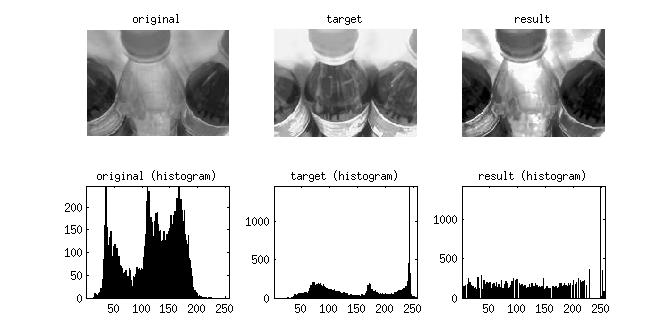
\includegraphics[scale=0.65]{figures/1-6.jpg}
    \caption{Histograms of the matching result}
    \label{fig:1-6}
\end{figure}

% 1.7
\subsection{Matching Algorithm Comparison}
Here we see the results of the previously discussed algorithm, the
implementation of which can be reviewed in \ref{appendix:histmatch}, in
comparison with the built-in MatLab function \code{histeq}.

\begin{figure}[H]
    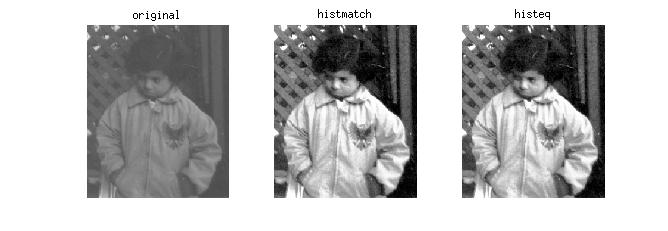
\includegraphics[scale=0.65]{figures/1-7.jpg}
    \caption{Comparison of histogram matching algorithms}
    \label{fig:1-7}
\end{figure}

The program used to generate this figure can be reviewed in \ref{appendix:1-7}

% 1.8
\subsection{Prove the Midway}
I didn't have time to do this one.

% 1.9
\subsection{Simplistic Midway Algorithm}
If we employ the more simplistic mathematical description of the algorithm,
we can generalize it for a sequence of $N$ images. Such an algorithm would
simply calculate the average across all the cumulative histograms in the
sequence.
\begin{align}
    C_m(x) = \frac{1}{N} \sum_{i=0}^{N}C_i(x)
\end{align}

An implementation of the midway specification can be reviewed in
\ref{appendix:midway}.
